% ::setlocal makeprg=cd\ latex\ &&\ pdflatex\ -interaction=batchmode\ main.tex\ &&\ xdg-open\ main.pdf\ &&\ exit
\chapter{Beautiful Closed Orbits}
\label{app:beautiful}

Once the integral of the precession has been expressed in terms of elliptic
integrals (eq. \ref{cap2:eq:delta_phi_elliptic}), we used a bisection algorithm
that allowed us to find the right value of $\hat \ell$ and
$\mathcal E$ that give a precession of exactly $\pi$, $\frac{\pi}{2}$,
$\frac{\pi}{3}$, etc.
The beautiful results are shown in the figures below.

\begin{figure}[h]
    \centering
    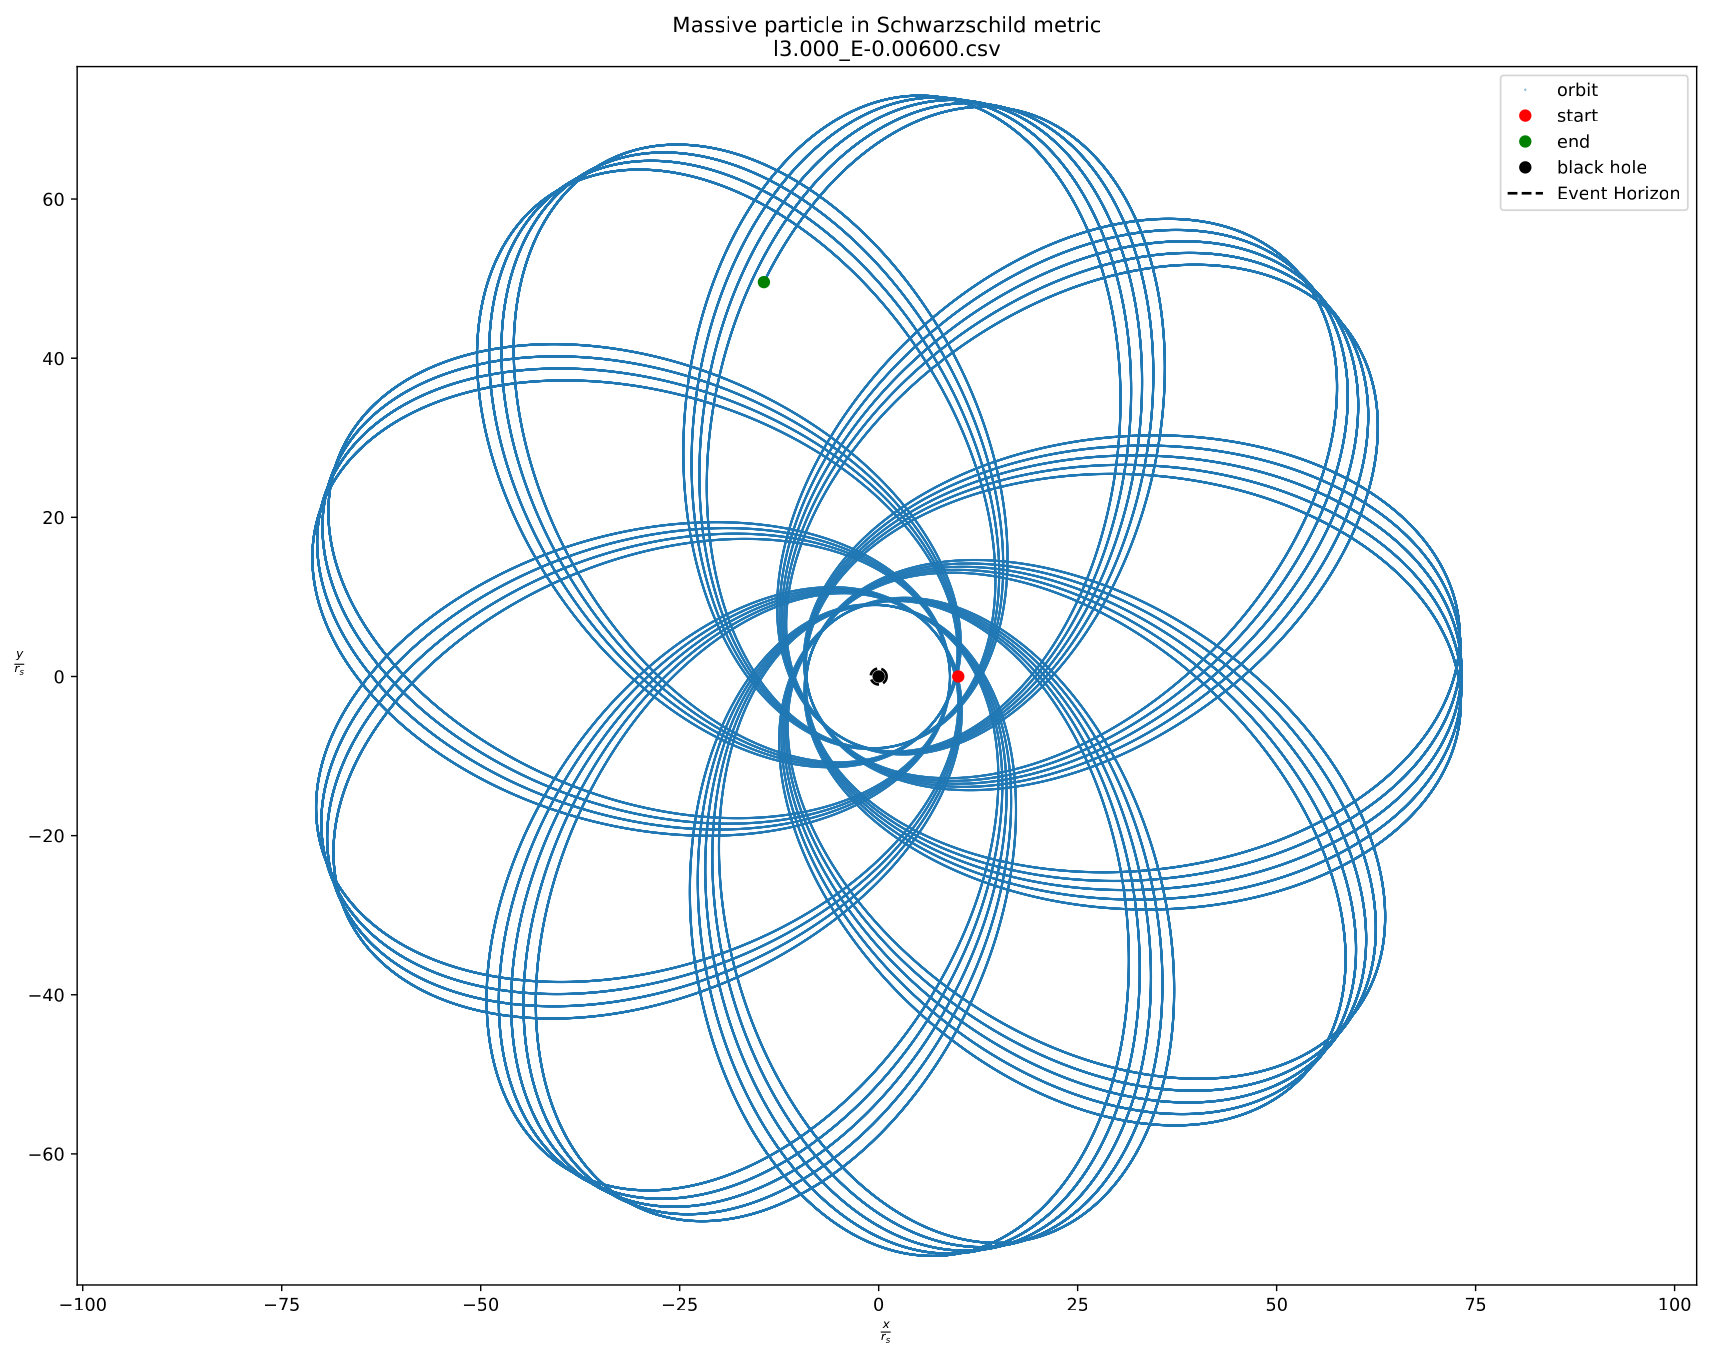
\includegraphics[width=\textwidth]{Figures/chapter2/wow0.png}
    \caption{[Placeholder] Not actually a closed orbit.}
    \label{cap2:fig:wow0}
\ oneend{figure}
%\begin{figure}[h]
%    \centering
%    \includegraphics[width=0.8\textwidth]{figures/elliptic_integral_1.eps}
%    \caption{\texttt{./main.x }}
%    \label{cap2:fig:wow1}
%\end{figure}
%
%\begin{figure}[h]
%    \centering
%    \includegraphics[width=0.8\textwidth]{figures/elliptic_integral_2.eps}
%    \caption{\texttt{./main.x }}
%    \label{cap2:fig:wow2}
%\end{figure}
%
%\begin{figure}[h]
%    \centering
%    \includegraphics[width=0.8\textwidth]{figures/elliptic_integral_3.eps}
%    \caption{\texttt{./main.x }}
%    \label{cap2:fig:wow3}
%\end{figure}
%
%\begin{figure}[h]
%    \centering
%    \includegraphics[width=0.8\textwidth]{figures/elliptic_integral_4.eps}
%    \caption{\texttt{./main.x }}
%    \label{cap2:fig:wow4}
%\end{figure}
